% 包含ctexbeamer文档类
\documentclass[t, aspectratio=169]{ctexbeamer}

%~~~~~~~~~~~~~~~~~~~~~~~~~~~~~~~~~~~~~~~~~~~~~~~~~~~~~~~~~~~~~~~~~~~~~~~~~~~~~~
% Define where theme files are located. ('/styles')
\usepackage{styles/nwafufluxmacros}
\usefolder{styles}
% Use Flux theme v0.1 beta
% Available style: asphalt, blue, red, green, gray 
\usetheme[style=asphalt]{nwafuflux}
%~~~~~~~~~~~~~~~~~~~~~~~~~~~~~~~~~~~~~~~~~~~~~~~~~~~~~~~~~~~~~~~~~~~~~~~~~~~~~~

%~~~~~~~~~~~~~~~~~~~~~~~~~~~~~~~~~~~~~~~~~~~~~~~~~~~~~~~~~~~~~~~~~~~~~~~~~~~~~~
% 载入需要的宏包
% 加载宏包
%===================注意======================%
% 在调用beamer.cls宏包后,以下宏包将自动调用,
% 不应单独调用这些宏包,以免发生冲突
% amsfonts, amsmath, amssymb, amsthm, 
% enumerate, geometry, graphics, graphicx, 
% hyperref, url, 
% ifpdf, keyval, xcolor, xxcolor
% =============================================%

% 参考文献宏包
% \usepackage[backend=biber,autolang=hyphen,style=gb7714-2015ay,
% doi=false,url=false,isbn=false]{biblatex}
\usepackage[backend=biber,autolang=hyphen,style=gb7714-2015,
gbtype=true,gbalign=gb7714-2015,
doi=false,url=false,isbn=false]{biblatex}

% Extra packages for the demo:
\usepackage{booktabs}
\usepackage{colortbl}
\usepackage{ragged2e}
\usepackage{schemabloc}

% 加载需要的宏包
\usepackage{csquotes}

% 符号字体
\usepackage{fontawesome5}

%%% Local Variables: 
%%% mode: latex
%%% TeX-master: "../main.tex"
%%% End:


% 进行必要的设置
% 载入字体(需要安装相应字体)
\setmainfont{LibertinusSerif}[% 英文字体
  Extension      = .otf,
  UprightFont    = *-Regular,
  BoldFont       = *-Bold,
  ItalicFont     = *-Italic,
  BoldItalicFont = *-BoldItalic,
  Scale          = 1.0]
\setmonofont{Iosevka}[Scale=1.0]% 等宽字体,主要用于代码排版
\setmathfont{LibertinusMath-Regular.otf}% Iosevka数学字体,需要unicode-math支持
\setCJKmainfont{Source Han Serif SC}[ % 中文衬线字体,思源宋体
  UprightFont     = * SemiBold,
  BoldFont        = * Heavy,
  ItalicFont      = * Light,
  BoldItalicFont  = * Medium,
  RawFeature      = +fwid]
\setCJKsansfont{Source Han Sans SC}[ % 中文无衬线字体,思源宋体
  UprightFont     = * Medium,
  BoldFont        = * Heavy,
  ItalicFont      = * Light,
  BoldItalicFont  = * Normal,
  RawFeature      = +fwid]  
\setCJKmonofont{Sarasa Mono SC}[% 中文等宽字体,Sarasa Mono SC
  UprightFont     = * Medium,
  BoldFont        = * Medium,
  ItalicFont      = * Extralight,
  BoldItalicFont  = * Light,
  RawFeature      = +fwid]   
% 也可以直接使用字体名称加载中文字体,思源字体,请将字体置于fonts目录下
% \setCJKmainfont[Extension=.otf,
%     Path=fonts/,
%     UprightFont=NotoSerifCJKsc-Regular,
%     BoldFont=NotoSerifCJKsc-Bold,
%     ItalicFont=NotoSerifCJKsc-Regular,
%     BoldItalicFont=NotoSerifCJKsc-Bold,
%     ItalicFeatures=FakeSlant,
%     BoldItalicFeatures=FakeSlant]{NotoSerifCJKsc}
% % 无衬线字体,思源字体,请将字体置于fonts目录下         
% \setCJKsansfont[
%     Extension=.otf,
%     Path=fonts/,
%     UprightFont=NotoSansCJKsc-Regular,
%     BoldFont=NotoSansCJKsc-Bold,
%     ItalicFont=NotoSansCJKsc-Regular,
%     BoldItalicFont=NotoSansCJKsc-Bold,
%     ItalicFeatures=FakeSlant,
%     BoldItalicFeatures=FakeSlant]{NotoSansSC}
% % 中文等宽字体,思源字体,请将字体置于fonts目录下  
% \setCJKmonofont[
%     Extension=.otf,
%     Path=fonts/,
%     UprightFont=NotoSansMonoCJKsc-Regular,
%     BoldFont=NotoSansMonoCJKsc-Bold,
%     ItalicFont=NotoSansMonoCJKsc-Regular,
%     BoldItalicFont=NotoSansMonoCJKsc-Bold,
%     ItalicFeatures=FakeSlant,
%     BoldItalicFeatures=FakeSlant]{NotoSansMonoSC}

%% 自定义相关的名称宏命令
%% ==================================================
%% \newcommand{\yourcommand}[参数个数]{内容}
% 西北农林科技大学各单位名称
\newcommand{\nwafu}{西北农林科技大学}
\newcommand{\cie}{信息工程学院}
\newcommand{\ca}{农学院}
\newcommand{\cpp}{植物保护学院}
\newcommand{\ch}{园艺学院}
\newcommand{\cast}{动物科技学院}
\newcommand{\cvm}{动物医学院}
\newcommand{\cf}{林学院}
\newcommand{\claa}{风景园林艺术学院}
\newcommand{\cnre}{资源环境学院}
\newcommand{\cwrae}{水利与建筑工程学院}
\newcommand{\cmee}{机械与电子工程学院}
\newcommand{\cfse}{食品科学与工程学院}
\newcommand{\ce}{葡萄酒学院}
\newcommand{\cls}{生命科学学院}
\newcommand{\cs}{理学院}
\newcommand{\ccp}{化学与药学院}
\newcommand{\cem}{经济管理学院}
\newcommand{\cm}{马克思主义学院}
\newcommand{\dfl}{外语系}
\newcommand{\iec}{创新实验学院}
\newcommand{\ci}{国际学院}
\newcommand{\dpe}{体育部}
\newcommand{\cvae}{成人教育}
\newcommand{\iswc}{水土保持研究所}

%% 签署春秋学期日期命令
\newcommand{\tomonth}{
  \the\year 年\the\month 月
}


\newcommand{\tomonthen}{
  \ifcase\the\month
  \or January%
  \or February%
  \or March%
  \or April%
  \or May%
  \or June%
  \or July%
  \or August%
  \or September%
  \or October%
  \or November%
  \or December%
  \fi, \the\year
}

\newcommand{\tosemester}{
  \the\year 年\ 
  \ifcase\the\month
  \or 秋%
  \or 春%
  \or 春%
  \or 春%
  \or 春%
  \or 春%
  \or 春%
  \or 夏%
  \or 秋%
  \or 秋%
  \or 秋%
  \or 秋%
  \fi 
}

\newcommand{\tosemesteren}{  
  \ifcase\the\month
  \or Autumn%
  \or Spring%
  \or Spring%
  \or Spring%
  \or Spring%
  \or Spring%
  \or Summer%
  \or Autumn%
  \or Autumn%
  \or Autumn%
  \or Autumn%
  \or Autumn%
  \fi, \the\year
}

% 插图路径设置
% ==================================================
\graphicspath{{figs/}}%图片所在的目录
% ==================================================

% 载入需要的TiKZ库
\usetikzlibrary{chains}

%% 设置绘制目录结构的宏及参数
\usepackage[edges]{forest}
\definecolor{folderbg}{RGB}{124,166,198}
\definecolor{folderborder}{RGB}{110,144,169}
\newlength\Size
\setlength\Size{4pt}
\tikzset{%
  folder/.pic={%
    \filldraw [draw=folderborder, top color=folderbg!50, bottom color=folderbg] (-1.05*\Size,0.2\Size+5pt) rectangle ++(.75*\Size,-0.2\Size-5pt);
    \filldraw [draw=folderborder, top color=folderbg!50, bottom color=folderbg] (-1.15*\Size,-\Size) rectangle (1.15*\Size,\Size);
  },
  file/.pic={%
    \filldraw [draw=folderborder, top color=folderbg!5, bottom color=folderbg!10] (-\Size,.4*\Size+5pt) coordinate (a) |- (\Size,-1.2*\Size) coordinate (b) -- ++(0,1.6*\Size) coordinate (c) -- ++(-5pt,5pt) coordinate (d) -- cycle (d) |- (c) ;
  },
}
\forestset{%
  declare autowrapped toks={pic me}{},
  declare boolean register={pic root},
  pic root=0,
  pic dir tree/.style={%
    for tree={%
      folder,
      %font=\ttfamily,
      grow'=0,
      s sep=1.0pt,
      font=\small \sffamily,
      %fit=band,
      %ysep = 1.0pt,
      inner ysep = 2.6pt,
    },
    before typesetting nodes={%
      for tree={%
        edge label+/.option={pic me},
      },
      if pic root={
        tikz+={
          \pic at ([xshift=\Size].west) {folder};
        },
        align={l}
      }{},
    },
  },
  pic me set/.code n args=2{%
    \forestset{%
      #1/.style={%
        inner xsep=2\Size,
        pic me={pic {#2}},
      }
    }
  },
  pic me set={directory}{folder},
  pic me set={file}{file},  
}
%% ==================================================

%%% Local Variables: 
%%% mode: latex
%%% TeX-master: "../main.tex"
%%% End: 

% ~~~~~~~~~~~~~~~~~~~~~~~~~~~~~~~~~~~~~~~~~~~~~~~~~~~~~~~~~~~~~~~~~~~~~~~~~~~~~~

% ~~~~~~~~~~~~~~~~~~~~~~~~~~~~~~~~~~~~~~~~~~~~~~~~~~~~~~~~~~~~~~~~~~~~~~~~~~~~~~
% 载入参考文献数据库
\addbibresource[location=local]{demo.bib}
% ~~~~~~~~~~~~~~~~~~~~~~~~~~~~~~~~~~~~~~~~~~~~~~~~~~~~~~~~~~~~~~~~~~~~~~~~~~~~~~

%~~~~~~~~~~~~~~~~~~~~~~~~~~~~~~~~~~~~~~~~~~~~~~~~~~~~~~~~~~~~~~~~~~~~~~~~~~~~~~
% Informations
\title[Flux Beamer 主题] % (可选,仅当标题过长时使用)
{西北农林科技大学 {\LaTeX}  Beamer 主题}

\subtitle{扁平主题 V\ 2.0}

\date{\tosemester} % 也可以使用类似\date[2017/04/20]{\zhdate{2017/04/20}}的
              % 方式指定时间

\author[N. Geng] % (可选,仅当有多个作者时使用)
{耿楠}

\institute[
智能媒体] % 可选项,在每页边栏的底部显示
{% 显示在标题页
  \cie
}

\titlegraphic{nwafulogo/cir_bar_h.pdf}
%~~~~~~~~~~~~~~~~~~~~~~~~~~~~~~~~~~~~~~~~~~~~~~~~~~~~~~~~~~~~~~~~~~~~~~~~~~~~~~

\begin{document}

% 标题页
\titlepage
% 目录页
\begin{frame}[allowframebreaks]{目录}{主讲内容}
 \tableofcontents
\end{frame}

\section{演示文稿}

\subsection{简介}

\begin{frame}{Flux主题}{简介}
  \justifying
  Flux是一个现代Beamer演示文稿主题,目前正在开发,并且可能不同版本间
  存在不一致性。 该主题托管于:\\[0.3cm]
  \centering\textbf{github.com/pvanberg/flux-beamer}
\end{frame}

\def\beamer@mytheme@style{green}
\begin{frame}[fragile]{Flux主题}{颜色设置}
  \centering
  Flux主题提供了5种颜色模式。\\
  \verb+\usetheme[style=asphalt]{flux}+\\[0.8cm]
  \newcommand{\colorRow}[1]{
    \begin{tabular}{p{4cm}cccc}
      #1 & \cellcolor{primary}\hspace*{1cm} &\cellcolor{primaryLight}\hspace*{1cm}&\cellcolor{secondary}\hspace*{1cm}&\cellcolor{tertiary}\hspace*{1cm}\\
    \end{tabular}
  }
  \colorRow{Asphalt}\\[0.3cm]
  \definecolor{primaryLight}{HTML}{3a99d9}
  \definecolor{primary}{HTML}{2e81b7}
  \definecolor{secondary}{HTML}{2e81b7}
  \definecolor{tertiary}{HTML}{e76d55}
  \colorRow{Blue}\\[0.3cm]
  \definecolor{primaryLight}{HTML}{77933c}
  \definecolor{primary}{HTML}{4f622a}
  \definecolor{secondary}{HTML}{884F4D}
  \definecolor{tertiary}{HTML}{2B3234}
  \colorRow{Green}\\[0.3cm]
  \definecolor{primaryLight}{HTML}{C0392B}
  \definecolor{primary}{HTML}{96281B}
  \definecolor{secondary}{HTML}{347986}
  \definecolor{tertiary}{HTML}{56423e}
  \colorRow{Red}\\[0.3cm]
  \definecolor{primaryLight}{HTML}{616161}
  \definecolor{primary}{HTML}{424242}
  \definecolor{secondary}{HTML}{518071}
  \definecolor{tertiary}{HTML}{8b7687}
  \colorRow{Gray}\\[0.3cm]
\end{frame}

\subsection{字体}

\begin{frame}[fragile]{Flux主题}{字体}
  Flux主题的排版默认效果:
  \begin{itemize}
  \item Regular
  \item \alert{Alert}
  \item \example{Example}
  \item \textit{Italic}
  \item \textbf{Bold}
  \end{itemize}        
\end{frame}

\subsection{脚注}

\begin{frame}{Flux主题}{脚注}
  Flux主题集成了自定义脚注。例如,为\textbf{这个素材}\footnote{脚注是放
    在页面底部的注释,用于引用参考文献或说明指定文本。例如,假设要为编
    写的句子添加有趣的注释,但注释与段落没有直接关系。},或是
  \textbf{另外素材}\footnote{脚注不只是为了有趣的注释,有时只是提供文本来
    源---以让读者知道这些材料来自何处,或者可以在哪里寻找有关该主题的其他来源。}提供一个脚注。
\end{frame}

\section{其它}
\subsection{列表}

\begin{frame}{Flux主题}{列表}
  \begin{columns}[T,onlytextwidth]
    \column{0.33\textwidth} \textbf{Items}
    \begin{itemize}
    \item 猫
    \item 狗
    \item 鸟
    \end{itemize}

    \column{0.33\textwidth} \textbf{Enumerations}
    \begin{enumerate}
    \item 第1个
    \item 第2个
    \item 第3个
    \end{enumerate}

    \column{0.33\textwidth} \textbf{Descriptions}
    \begin{description}
    \item[苹果] 是
    \item[橙子] 否
    \item[葡萄] 否
    \end{description}
  \end{columns}
  \let\thefootnote\relax\footnote{注意:以下slides直接摘录于metropolis
    主题。 Copyright 2014 Matthias Vogelgesang.\\
    详见https://github.com/matze/mtheme/tree/master/demo}
\end{frame}

\subsection{表格}

\begin{frame}{Flux主题}{表格}
  \begin{table}
    \caption{世界上最大的城市(来源: Wikipedia)}
    \begin{tabular}{@{} lr @{}}
      \toprule
      City & Population\\
      \midrule
      Mexico City & 20,116,842\\
      Shanghai & 19,210,000\\
      Peking & 15,796,450\\
      Istanbul & 14,160,467\\
      \bottomrule
    \end{tabular}
    \hspace*{1cm}
        \setlength\extrarowheight{3pt}
    \begin{tabular}{|lr|}
      \hline
      \rowcolor{primaryLight}\color{background}City & \color{background}Population\\
      \hline
      Mexico City & 20,116,842\\
      Shanghai & 19,210,000\\
      Peking & 15,796,450\\
      Istanbul & 14,160,467\\
      \hline
    \end{tabular}
\end{table}
\end{frame}

\subsection{区块}

\begin{frame}[fragile]{Flux主题}{区块}
  Flux主题设计了3个预定义的区块样式。\\
  用\verb+\setblockstyle{native}+调用默认的Native样式。\\[0.5cm]
  
  \setblockstyle{native} % 默认行为
  \begin{center}
    \begin{minipage}[b]{0.5\textwidth}
      \begin{block}{默认区块}
        区块内容。
      \end{block}

      \begin{alertblock}{警示区块}
        区块内容。
      \end{alertblock}

      \begin{exampleblock}{示例区块}
        区块内容。
      \end{exampleblock}
    \end{minipage}
  \end{center}
\end{frame}

\begin{frame}[fragile]{Flux主题}{区块}
  Flux主题设计了3个预定义的区块样式。\\
  用\verb+\setblockstyle{nobackground}+调用默认的NoBackground样式。\\[0.5cm]
  
  \setblockstyle{nobackground} % 默认行为
  \begin{center}
  \begin{minipage}[b]{0.5\textwidth}
    \begin{block}{默认区块}
      区块内容。
    \end{block}

    \begin{alertblock}{警示区块}
      区块内容。
    \end{alertblock}

    \begin{exampleblock}{示例区块}
      区块内容。
    \end{exampleblock}
  \end{minipage}
  \end{center}
\end{frame}

\begin{frame}[fragile]{Flux主题}{区域}
  Flux主题设计了3个预定义的区块样式。\\
  用\verb+\setblockstyle{metropolis}+调用默认的Metropolis样式。\\[0.5cm]
  
  \setblockstyle{metropolis}
  \begin{center}
    \begin{minipage}[b]{0.5\textwidth}
      \begin{block}{默认区块}
        区块内容。
      \end{block}

      \begin{alertblock}{警示区块}
        区块内容。
      \end{alertblock}
    
      \begin{exampleblock}{示例区块}
        区块内容。
      \end{exampleblock}
    \end{minipage}
  \end{center}
\end{frame}

\begin{frame}{Flux主题}{插图}
  \centering
  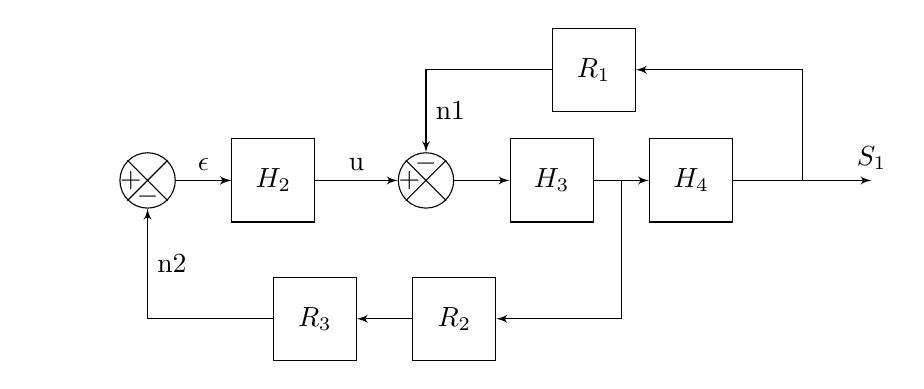
\begin{tikzpicture}
    \sbEntree{E}
    \sbComp{a}{E}
    \sbBlocL{c}{$H_2$}{a}
    \sbRelier[$\epsilon$]{a}{c}
    \sbComph{d}{c}
    \sbRelier[u]{c}{d}
    \sbBlocL{e}{$H_3$}{d}
    \sbBlocL{f}{$H_4$}{e}
    \sbSortie[5]{S1}{f}
    \sbRelier{f}{S1}
    \sbNomLien[0.8]{S1}{$S_1$}
    \sbDecaleNoeudy[-4]{f}{u}
    \sbDecaleNoeudy{e}{v}
    \sbBlocr{r1}{$R_1$}{u}
    \sbBlocr{r2}{$R_2$}{v}
    \sbBlocrL{r3}{$R_3$}{r2}
    \sbRelieryx{f-S1}{r1}
    \sbRelierxy[n1]{r1}{d}
    \sbRelieryx{e-f}{r2}
    \sbRelierxy[n2]{r3}{a}
  \end{tikzpicture}\\[0.4cm]
  插图示例来自于\textbf{texample.net}
\end{frame}

\begin{frame}{Flux主题}{绘图}
  \begin{minipage}{0.58\textwidth}
    \begin{figure}
      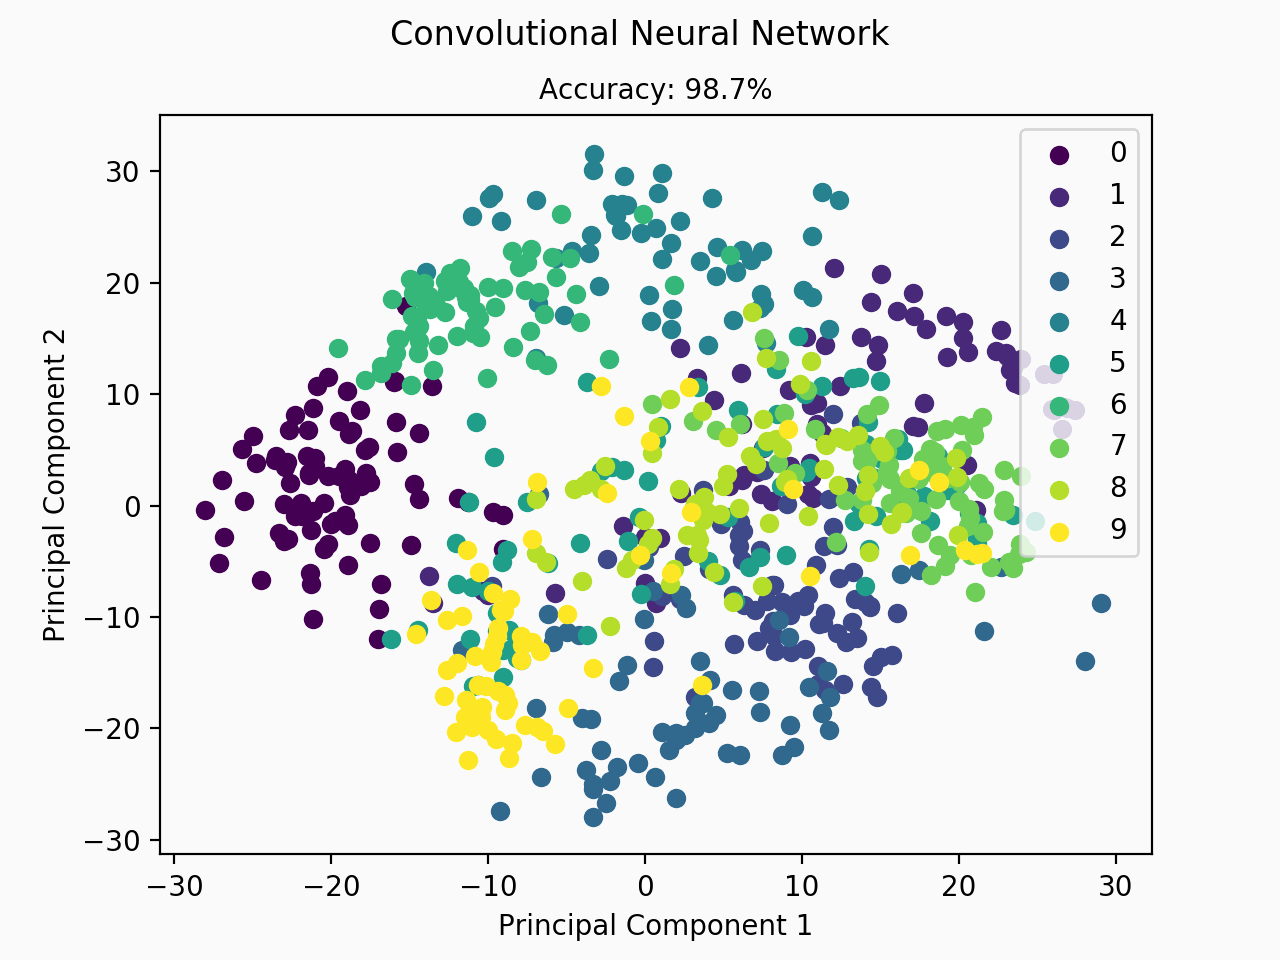
\includegraphics[width=\textwidth]{figs/plot.png}
    \end{figure}
  \end{minipage}
  \hfill
  \centering
  \begin{minipage}{0.4\textwidth}
    \begin{block}{二元Softmax分类器}
      \centering $\sigma(\sum_i w_ix_i + b)$
    \end{block}
    \begin{exampleblock}{损失函数}
      \centering\vspace*{0.1cm}
      $L_i = -log(\frac{e^{f_{y_i}}}{\sum_j e^{f_j}})$\\[0.1cm]
      交叉熵
    \end{exampleblock}
  \end{minipage}
\end{frame}

% [plain]参数可以禁用headlines、footlines和sidebars,
% 用于显示大图片、进行强调等
\begin{frame}[plain]
  \begin{center}
    这是一个plain帧。\\
    可以用于显示大图片、进行强调等。
  \end{center}
\end{frame}

\begin{frame}[allowframebreaks]{参考文献}{文献列表}
  \nocite{*}  
  \printbibliography[heading=bibliography,title=参考文献]
\end{frame}

\section{下一节}
\subsection{小节1}
\subsection{小节2}
\subsection{小节3}
\section{更多节}
\subsection{小节1}
\subsection{小节2}
\subsection{小节3}

\section{问题反馈}
\subsection{错误, 意见和建议}
% 问题、意见和建议
\begin{frame}{问题反馈}{错误、意见和建议}
  \begin{itemize}
  \item 本主题中会存在错误,如果发现了错误,请联系我进行改进
    \begin{itemize}
    \item \alert{再小的问题也是问题}
    \end{itemize}
  \item 如果你有好建议和使用体验改善意见,请联系我进行改进
  \end{itemize}
\end{frame}
%%%%%%%%%%%%%%%%

%%%%%%%%%%%%%%%%%%%%%%%%%%%%%% 关于我们 %%%%%%%%%%%%%%%%%%%%%%%%%%%%%%%%%%%
\section[关于我们]{关于我们}
\subsection[联系方式]{联系方式}
\begin{frame}[fragile]{关于我们}{联系方式}
  % colour options
  \definecolor{seplinecolour}{HTML}{357f2d} % green
  \definecolor{iconcolour}{HTML}{2f3142} % dark
  \definecolor{textcolour}{HTML}{2f3142} % dark
  \definecolor{jobtitlecolour}{HTML}{474a65} % light dark

  % define some lengths for internal spacing
  \newlength{\seplinewidth} \setlength{\seplinewidth}{2cm}
  \newlength{\seplineheight} \setlength{\seplineheight}{1pt}
  \newlength{\seplinedistance} \setlength{\seplinedistance}{0.3cm}
  \begin{center}
      \begin{tikzpicture}[font=\small]
      % name
      \matrix[every node/.style={anchor=center,font=\huge},anchor=center] (name) {
        \node{耿\hspace{\ccwd}楠}; \\
        %\node{\color{jobtitlecolour}\normalsize\textit{教授}}; \\
      };
      % sep line 1
      \node[below=0.3\seplinedistance of name] (hl1) {};
      \draw[line width=\seplineheight,color=seplinecolour] (hl1)++(-\seplinewidth/2,0) -- ++(\seplinewidth,0);
      % contact info
      \matrix [below=\seplinedistance of hl1,%
               column 1/.style={anchor=center,color=iconcolour},%
               column 2/.style={anchor=west}] (contact) {
        \node{\faGlobe}; & \node{\url{http://cie.nwsuaf.edu.cn/szdw/}};\\
        \node{\faBuilding}; & \node{西北农林科技大学信息工程学院计算机科学系};\\ 
        \node{\faEnvelope}; & \node{nangeng@nwafu.edu.cn; nangeng@qq.com};\\
        %\node{\faQq}; & \node{970291228};\\
        %\node{\faPhone}; & \node{15829540966}; \\
        \node{\faGithub}; & \node{\url{https://github.com/registor/}}; \\
      };
      sep line 2
      \node[below=\seplinedistance of contact] (hl2) {};
      \draw[line width=\seplineheight,color=seplinecolour] (hl2)++(-\seplinewidth/2,0) -- ++(\seplinewidth,0);
      % interests
      \matrix [below=\seplinedistance of hl2,
         every node/.style={anchor=center,font=\Large}]
         (interests) {
        \node{\faCode}; & \node{\faCoffee}; &
        \node{\faLock}; & \node{\faWrench}; &
        \node{\faCameraRetro}; \\
      };
    \end{tikzpicture}
  \end{center}    
\end{frame}

% 封底
\begin{frame}[c,plain,noframenumbering]
  \centering
  谢谢你使用该{\LaTeX} Beamer主题!\\欢迎多提宝贵意见和建议!
\end{frame}

\end{document}
%%% Local Variables:
%%% mode: latex
%%% TeX-master: t
%%% End:
